\selectlanguage{english}

\section{MIMO- Basics}

\ac{MIMO} is a break through in wireless communication, that uses spatial dimension provided by the N transmit and M receive antennas to combat multipath fading. \ac{MIMO} has become an essential element of wireless communication standards including IEEE 802.11n (Wi-Fi), IEEE 802.11ac (Wi-Fi), and Long Term Evolution (4G).

A \acs{MIMO} network with N number of transmit and M number of receive antennas an extension of antenna array communication, that provides high spectral efficiency (The spectral efficiency can be defined by the total number of information bits per second per Hertz transmitted from one array to another), improves reliability and sensitivity to fading; reduced by spatial diversity that is provided by the multiple paths . There are several advantages of having \acs{MIMO} antennas like gain, spatial and transmit diversity. 

The figure represents a typical \ac{MIMO} system where multiple data streams are  transmitted in a single channel at the same time and multiple radios collect the multipath signals.

\begin{figure}[h]
	\begin{center}
		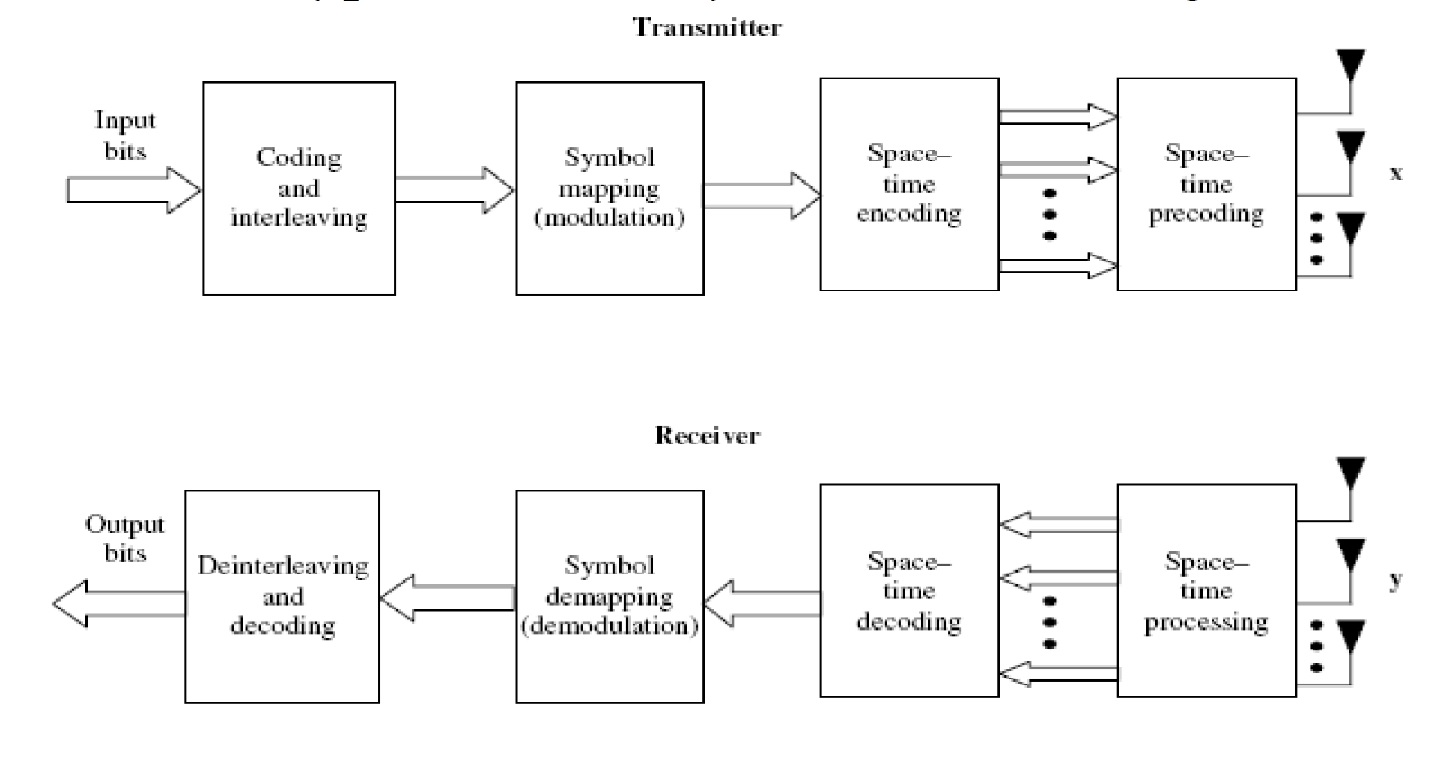
\includegraphics[width= 0.8\textwidth]{mimosystem.eps}
		\caption{MIMO System Model}
	\end{center}
\end{figure}


A typical \ac{MIMO} channel and system model equation is as represented as in equation 1. The wireless channel part can be seen in keenly with the received vector \me{y} can be represented in terms of the channel \me{H}. 

\begin{equation}
\mathbf{y} = H \mathbf{x} + n
\label{bgmimo1_eqn}
\end{equation}
where, transmitted signal vector \me{x = x_1,x_2, \dotsc,x_n}, recieved vector \me{y = y_1, y_2, \dotsc, y_n} and the channel matrix can be represented as, \me{H} =  \[ \left( \begin{array}{cccc} 
h_{11} & h_{12} & \dotsc & h_{1M} \\
h_{21} & h_{22} & \dotsc & h_{2M} \\
\dotsc & \dotsc & \dotsc & \dotsc \\
h_{N1} & h_{N2} & \dotsc & h_{NM} \end{array} \right)\].

The capacity for \ac{MIMO} defined in \cite{weingarten2004capacity}, network capacity can be written as
\begin{equation}
C = \underset{f(x)}{\text{max}} I(X;Y) 
\label{bgmimo2_eqn}
\end{equation} 
where, \me{I(X;Y)} is the mutual information of the channel represented as,
\begin{equation}
I(X;Y) = \int \log (\dfrac{f(y|x)}{f(y)}) dF(x,y)
\label{bgmimo3_eqn}
\end{equation}
\begin{figure}[h]
	\begin{center}
		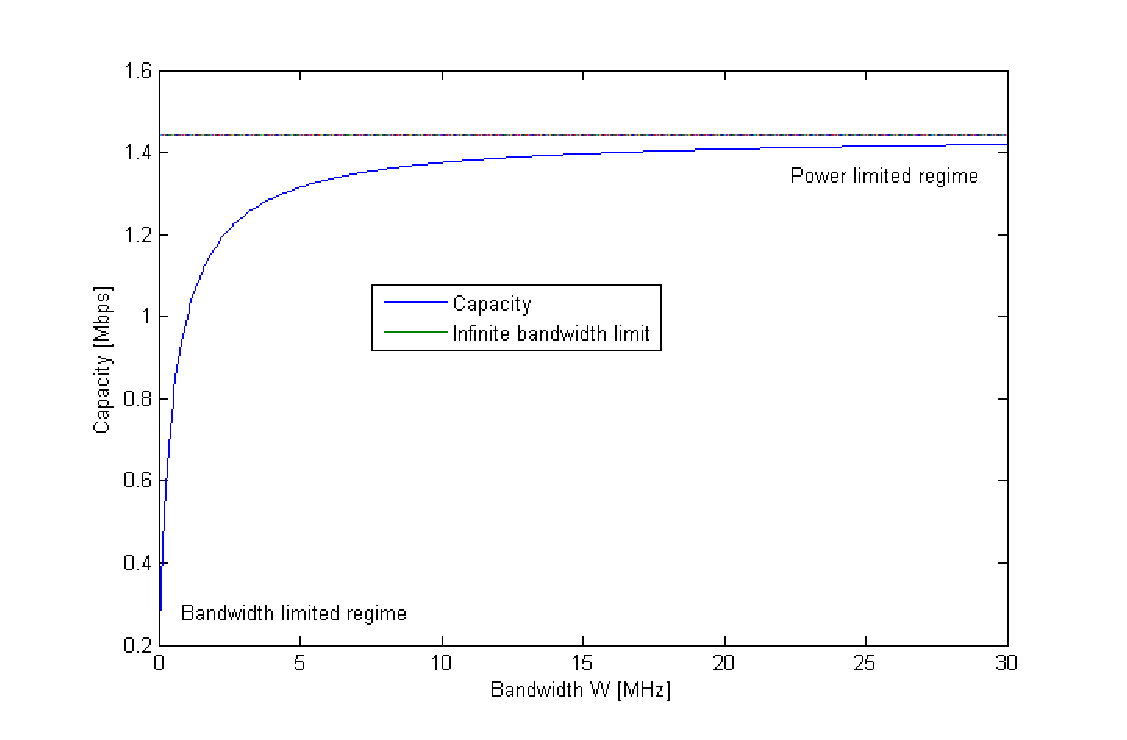
\includegraphics[width= 0.8\textwidth]{mimocapacity.eps}
		\caption{MIMO Capacity}
	\end{center}
\end{figure}
where the integral is taken over the random variables X and Y, \me{f(x)} and \me{f(y)} is denoted as the probability density function of X and Y, \me{F(x,y)} is the cumulative distribution function of X and Y respectively. The mutual Information can also be written in terms of differential output of channel entropy and the conditional entropy. 
\begin{equation}
I(X;Y) = h(Y) - h(Y|X)
\label{bgmimo4_eqn}
\end{equation}
For a time-invariant \ac{AWGN} channel with received \ac{SNR} \me{\gamma}, the maximizing input distribution is Gaussian, which results in the channel capacity	
\begin{equation}
C = \alpha \log (1 + \gamma)
\label{bgmimo5_eqn}
\end{equation}

At high \ac{SNR}, the capacity of the i.i.d. Rayleigh fast fading channel scales like \me{n_min \log} SNR bits/s/Hz, where \me{n_min} is the minimum of the number of transmit antennas \me{n_t} and receive antennas \me{n_r}. Thus, at high \ac{SNR} we obtain degree-of-freedom gain. At low \ac{SNR}, the capacity is approximately \me{n_r} SNR \me{\log_2}e bits/s/Hz. Thus at low \ac{SNR} what we obtain is the recieve beamforming power gain. At all \ac{SNR} the capacity increases linearly with \me{n_min} due to the linear combination of degree of freedom gain and beamforming power gain.

%The \ac{MIMO} information-theoretic performance bound of the system can be explained here while Capacity increases linearly at low \ac{SNR} but increases logarithmically at high \acs{SNR}. The linear region is the Bandwidth limited region and the logarithmic region is power limited region, since in low \ac{SNR} region the capacity which is defined as C = log (1 + SNR) where \ac{SNR} value is small so effectively we have log(1) like wise for high \ac{SNR} value the log(1 + SNR) term is effectively \ac{SNR} since for higher values log term increases slowly. 
%-----------------------------------------------------------------------------
%  MIMO ibc
%-----------------------------------------------------------------------------

\section{MIMO-IC}
\ac{MIMO} communication systems has been showing a great potential in increasing the average throughput in the wireless communication scenario. Due to the performance gain in channel capacity and spectral efficiency in point to point \ac{MIMO} systems has made the inclusion of singe user \ac{MIMO} in different communication stansards. SU-\ac{MIMO} has proved its efficiency to enhance the perormance in wireless networks. But, in cellular systems the available spectrum is very costly and is scarce so such systems has to deal with the inter-cell interference which doesnot exists in isolated point to point systems.

\begin{figure}[h]
	\begin{center}
		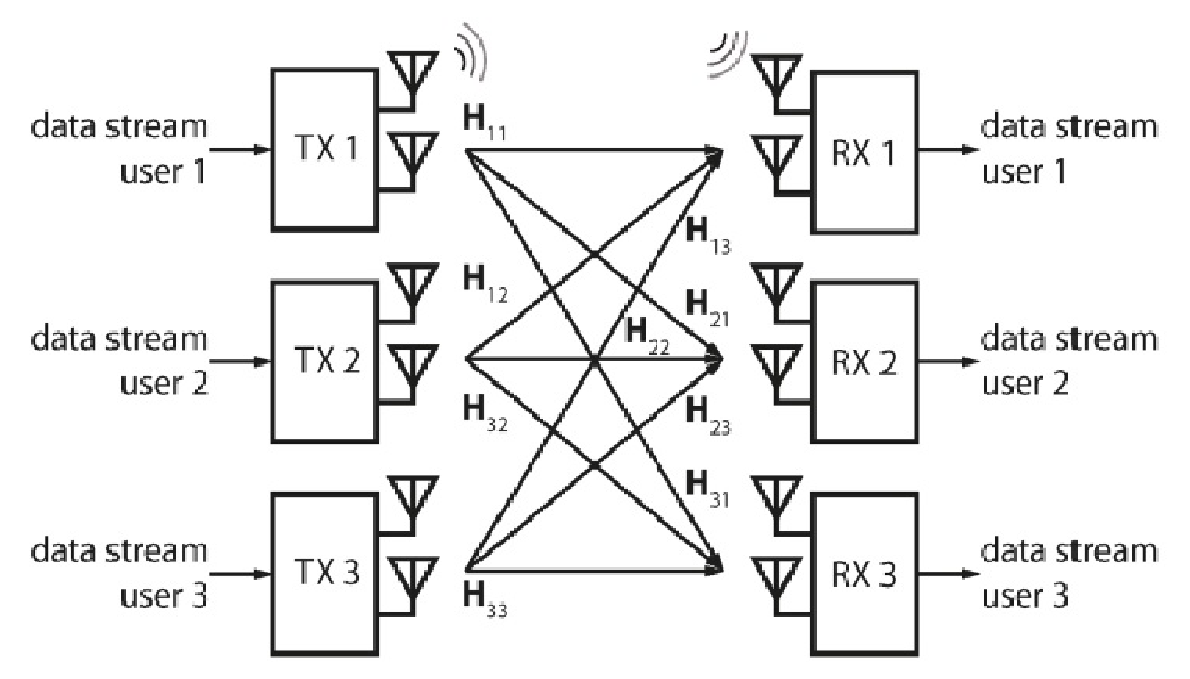
\includegraphics[width= 0.8\textwidth]{mimoibc.eps}
		\caption{MIMO-IC System Model}
	\end{center}
\end{figure}

Interference is a major set back and a limiting factor in the wireless communication networks. The problem of interference is in general  dealt  with  planning of the  (mostly  static) radio resource management. Now a days we have a popularity of wireless  devices  having  different  wireless  communication standards, the the ability to produce a desired or intended result of such interference avoidance solutions is limited. These days, standardization bodies are including  interference coordination strategies in  next generation  cellular  communication standards.  A  systematic study  of  the  performance of  cellular  communication systems where  each  cell  communicates  multiple  streams to  its  users while causing interference from and to the neighboring cells due  to  transmission  over  a  common  shared  resource  known as, \ac{MIMO}-\ac{IC}. A K-user \ac{MIMO}-\ac{IC} model consists of a network of K transmit-receive  pairs  where each transmitter  communicates  multiple data streams to its respective receiver. In doing so, it generates interference at all other receivers present in the system.

%-----------------------------------------------------------------------------
%  MIMO ibc
%-----------------------------------------------------------------------------


\section{MIMO-IBC}

The linear transceiver design problem is considered in a \ac{MIMO}-\ac{IBC}, in which a set of \ac{BS}s send data to their intended users. Both the \ac{BS}s and the users are equipped with multiple antennas, and they share the same time/frequency resource for transmission. The objective is to maximize the minimum rate among all the users in the network, in order to achieve fairness.

\begin{figure}[h]
	\begin{center}
		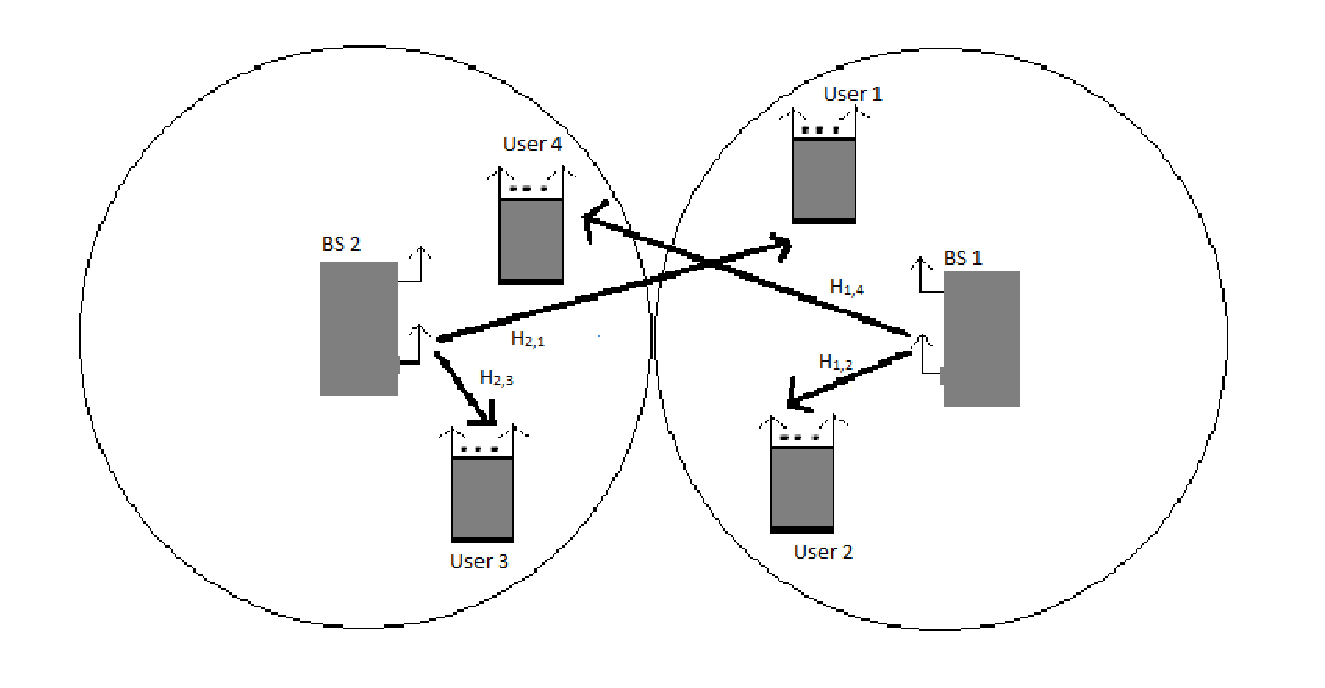
\includegraphics[width= 1.0\textwidth]{system_model.eps}
		\caption{MIMO-IBC System Model}
	\end{center}
\end{figure}

Interference is the main limiting factor in wireless transmission. \ac{BS} consisting of multiple antennas are able to serve multiple users simultaneously, which is the principle of \ac{SDMA} or \ac{MU-MIMO}. However, \ac{MU} systems have precise requirements for \ac{CSIT} which is more difficult to acquire than \ac{CSI} at the Rx \ac{CSIR}. Hence we focus here on the more challenging \ac{DL} (though the \ac{UL} is also non-trivial in the case of Mobile Terminals (MTs) with multiple antennas). In cellular systems, one can distinguish between the cell center where a single cell design is appropriate (due to high \ac{SIR} and the cell edge where a multi-cell approach is mandatory. The \ac{MU-MIMO} \ac{DL} problem for the cell center users is called the (MIMO) Broadcast Channel (BC). or the cell edge users,  the recent introduction of Interference Alignment (IA) has shown that approaching high system capacity through agressive frequency reuse should in principle be possible.  Whereas precise capacities for cellular systems remain unknown, IA allows to reach the optimal high \ac{SNR} rate prelog, called Degree of Freedom \ac{DoF} (or spatial multiplexing factor, or number of streams). That is, before accounting for \ac{CSI} acquisition.  

Optimal  precoder  design  for  \ac{WSRM} in \ac{MIMO} interference networks  is  studied.  For  this  well  known  non-convex  optimization problem, convex approximations based on interference alignment are developed, for multi-beam cases. Considering that each user treats interference from other users as noise. It is well known that, due to interference coupling, the problem is a non-convex optimization and is hard to solve. In the high \ac{SNR} regime, there has been recent progress on maximizing the sum degrees of freedom, exploiting the idea of interference alignment. It has been shown that maximizing the sum degrees of freedom is  still  an  NP  hard  problem. 


%-----------------------------------------------------------------------------
%  MATH
%-----------------------------------------------------------------------------


\section{Mathematical Preliminaries}
\subsection{Convex Optimization}

\subsubsection{Convexity}
Convexity is also called convex analysis, which is an area in mathematics where one studies about convex sets and convex functions. Convexity is also the mathematical core of optimization [1], where it plays an important role in statistics, differential equations and mathematical economics. Convexity can also be called as convex analysis. Some examples of convex sets are triangle, rectangle, polyhedron and quadratic equations.[1]. 
\begin{figure}[h]
	\begin{center}
		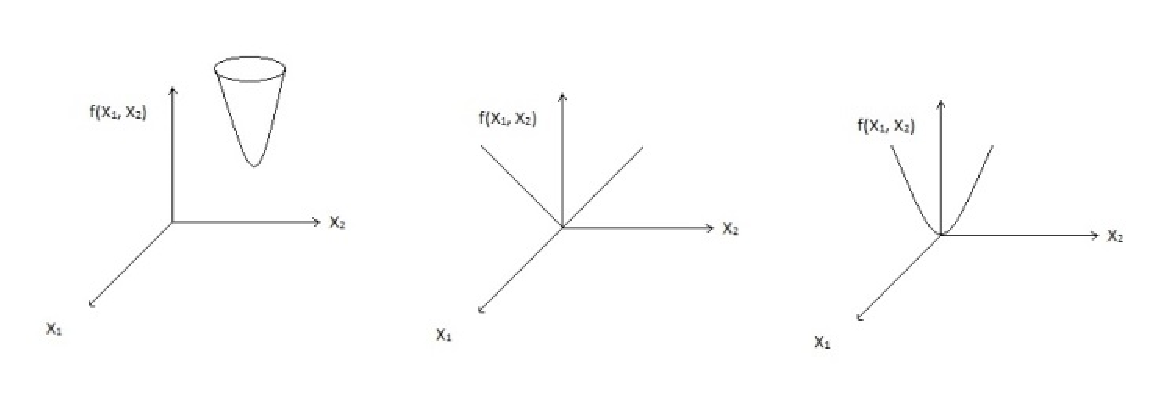
\includegraphics[width= 1.0\textwidth]{convexfunc.eps}
		\caption{Convex Functions}
	\end{center}
\end{figure}
\subsection{Convex Sets}
Consider \me{\mathcal{K}} is a set of \me{\mathcal{R}^n} is said to be convex when the line segment through the points \me{x, y} belongs to \me{\mathcal{K}}. In general, the points must lie inside the set and the set is connected such that without leaving the set we can pass through any two points. As mentioned above there are several examples for convex sets like ellipsoid, hypercubes etc. We can also define that the intersection of any convex sets is a convex set.[2]. 
A set that is not convex is called non convex set or also called as concave set. We can define a non convex set by considering a line segment joining the points \me{x, y} lies outside the set \me{\mathcal{K}}.
\begin{figure}[h]
	\begin{center}
		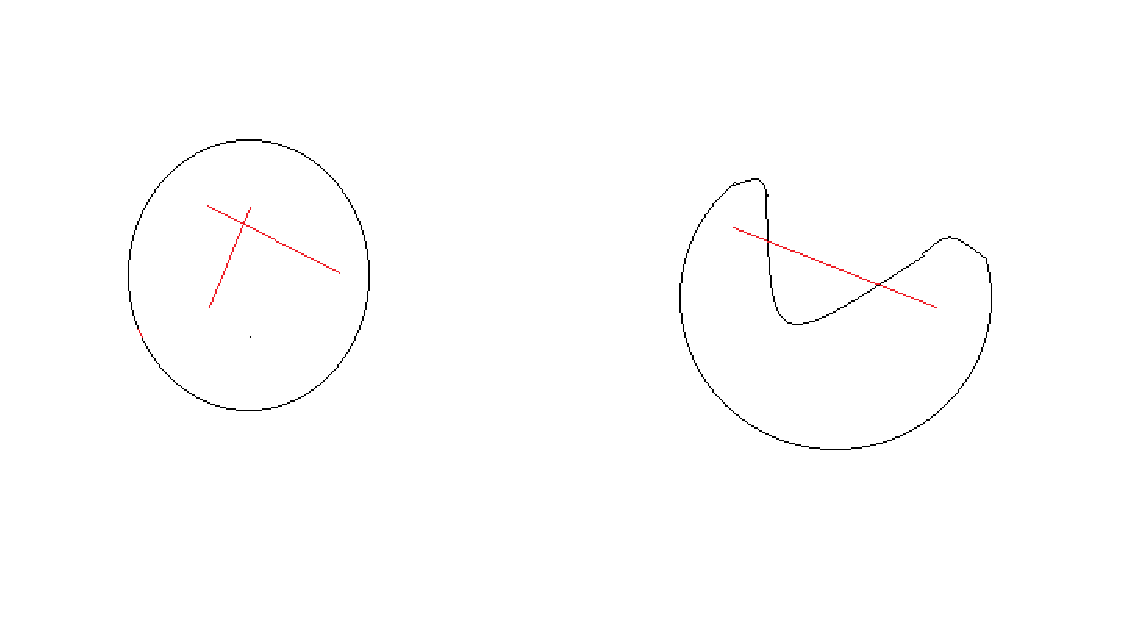
\includegraphics[width= 0.8\textwidth]{convexset.eps}
		\caption{Convex Sets}
	\end{center}
\end{figure}

\subsubsection{Convex Functions}

Convex functions are continuous function and is convex if and only if the region above the graph as shown in figure is convex set. A function \me{f} is convex if, \me{\forall} \me{x, y} \me{\in} \me{\mathcal{K}}, \me{ \forall} \me{ \theta \in} [0, 1]: 
\begin{equation}
f(\theta x + (1 - \theta) y) \leq \theta f(x) + (1 - \theta) f(y)
\end{equation}
The function \me{f} is said to be strictly convex if, \me{ \forall} \me{x \neq y} \me{\in} \me{\mathcal{K}}, \me{ \forall} \me{ \theta \in} (0, 1):
\begin{equation}
f(\theta x + (1 - \theta) y) < \theta f(x) + (1 - \theta) f(y)
\end{equation}
A function \me{f} is said to be concave if the function -\me{f} is strictly convex. Strict convexity means that the graph of \me{f} lies below the segment \me{\mathcal{S}}. Certain examples of strict convex functions are exponential and quadratic function. Several operations on these function preserves the convexity like summation, multiplication of convex functions. 

\subsubsection{Optimization Problem}

A generic optimization problem is similar to linear programming problem, that can be solved quickly depending on the variables and the constraints. The objective and the constraints must be linear for the problem to be convex. In general, a convex optimization problem has all of the constraints as convex functions, and the objective is a convex function of minimizing, or a concave function of maximizing. 

The standard form of optimization problem can be written as,
\begin{eqnarray}
\underset{x}{\text{minimize}} \quad && f(x) \\
\text{subject to} \quad && x \in \mathcal{X}. 
\end{eqnarray}
where, \me{f(x): {\mathbb{R}^n} \rightarrow {\mathbb{R}}} is the objective function that has to be minimized with respect to \me{x} and \me{\mathcal{X}} \me{\subset} \me{{\mathbb{R}^n}} is the feasible set. A maximization problem can be written by negating the objective function.

\subsubsection{Convex Problem}

A convex optimization problem is one which has both the objective and the given set of constraint as convex. In general linear functions are convex so the linear programming problem is convex problem. A general convex optimization problem can be written as
\begin{eqnarray}
\underset{x}{\text{minimize}} \quad && f(x) \\
\text{subject to} \quad && g_i(x) \leq 0, i = 1,...m\\
&& h_j(x) = 0, j = 1,...p.
\end{eqnarray}
where, \me{f(x): {\mathbb{R}^n} \rightarrow {\mathbb{R}}} is the objective function and \me{\mathcal{X}} \me{\subset} \me{{\mathbb{R}^n}} is the feasible set and is called convex when \me{\mathcal{X}} is closed convex set and \me{f(x)} is convex on \me{{\mathbb{R}^n}}. The second equation is the inequality constraint and the third is the equality constraint in the above optimization problem.
\par
The optimality condition for a convex problem; assume a feasible point \me{\mathbf{x}^*} but it is necessary to know if this point is the optimal solution. We can consider the gradient of a function \me{f} that shows the ascent direction of the function. Gradient of \me{f} at a point \me{x} divides the space into three regions one where the function increases, one where the function decreases and the one where we cannot figure out using the gradient alone. For \me{\mathbf{x}^*} to be optimal and the feasible region doesn't lie in the half space where the function decreases, if not then the point \me{\mathbf{x}^*} is not the optimal point. Convexity makes this condition sufficient for optimality. 
\par
To find solution for an unconstrained objective, we differentiate the objective function with respect to the optimization variable \me{x} and equate to zero as \me{\nabla f(x) = 0}. However for an constrained problem, we solve the Lagrangian as
\begin{equation}
\underset{\lambda}{\text{maximize}} \quad \underset{x}{\text{minimize}} \quad  L(x,\lambda_1, \dotsc,\lambda_m) =  f(x) + \lambda_1 g_1(x) + \dotsc + \lambda_m g_m(x) + \mu_1 h_1 (x) + \dotsc + \mu_p h_p(x),
\end{equation}
where \me{\lambda_i \geq 0} and \me{\mu_j} are Lagrange multipliers. In order to solve the constrained problem, similar to the unconstrained problem we take the partial derivative of the Lagrangian with respect to the optimization variable.
\par
When the objective is convex, and the equality conditions are affine and the inequality conditions are convex then one of the possible solutions, in some minimum principle is equivalent to \ac{KKT} optimality conditions. To solve a convex optimization problem as above with the \ac{KKT} approach we need the lagrange multiplier. There exists \me{\lambda_1, \lambda_2, \dotsc, \lambda_m, \mu_1, \dotsc, \mu_p}, called the Lagrange multipliers, for each point \me{x \in X} that minimizes f over \me{\mathcal{X}}. The Lagrange multipliers must satisfy certain conditions:\\
1. \me{{x} \quad minimizes \quad L(z, \lambda_1, \lambda_2, \dotsc, \lambda_m),   \forall z \in X},\\
2. \me{\lambda_1 \geq 0, \lambda_2 \geq 0, \dotsc, \lambda_m \geq 0},\\
3. Complementary Slackness: \me{\lambda_1 g_1 = 0, \lambda_2 g_2 = 0, \dotsc, \lambda_m g_m = 0}.\\
\par 
When the problem is has a convex objective and non convex constraint set then \ac{KKT} method is not a feasible approach. 


\subsubsection{Non Convex Problem}

A non convex problem is the one that has objective or any one of its constraint as non convex. Such problems have multiple feasible regions and multiple local minima in a region. An example for a non convex function would be a sine wave. Let us consider a non convex problem,
\begin{eqnarray}
\underset{x}{\text{minimize}} \quad && f(x) \\
\text{subject to} \quad && g_i(x) \leq 0, i = 1,\dotsc,m\\
&& h_j(x) = 0, j = 1,\dotsc,p.
\end{eqnarray} 
with variable \me{x \in \mathbb{R}^n}
\par
Let us consider a non convex problem when the objective function \me{f(x)} is convex and the inequality constraint \me{g_i(x)}, \me{i=1,\dotsc,n}  is differentiable convex function and \me{g_i(x)}  \me{i= (n+1),\dotsc,m} are differentiable function and the linearity constraint is affine. These non convex problems are common in wireless communication and this is our interest. In order to solve this problem the non convex part of the objective is approximated around a convex function to solve in an iterative manner. 
\par
As mentioned in the paper gordon.p. wright the inner approximation algorithm for the minimization problem can be done in the following steps,\\
\par
step 0. Set a starting point for the variable and constraint \me{x^0 \in F} and set \me{h^0 = g_0(x^0)}. Let \me{A^0 = \lbrace x|h^0 = g_0(x)} and \me{x \in F \rbrace}, where \me{F} can be defined as the feasible region.\\
\par
step 1. In the \me{k^{th}} iteration replace the constraint \me{g_i(x) \leq 0}, \me{i = (n+1), \dotsc, m}, by \me{\bar{g_i}(x,x^k) \leq 0}, where \me{\bar{g_i}(x,x^k)} is a differentiable convex function and \me{x^k \in \mathcal{A}^{k - 1}}. Each function \me{\bar{g_i}(x,x^k)} must  have the following properties,\\
1. \me{g_i(x) \leq \bar{g}_i(x,x^k) \quad \forall x \in {F}^k}\\
2. \me{g_i(x) = \bar{g_i(x^k,x^k)}}\\
3. \me{\delta g_i(x^k)/ \delta x_j =\delta \bar{g}_i(x^k,x^k)/\delta x_j \quad j=1,\dotsc,n}\\
The feasible region \me{F^k = \lbrace x|g_i(x) \leq 0 \forall i= 1,\dotsc , n} and \me{\bar{g}_i(x,x^k) \leq 0 \forall i= n+1, \dotsc, m \rbrace} should satisfy slaters constraint qualification condition for convex programs.\\
\par
step 2. Solve the approximation convex program\\

\begin{eqnarray}
\underset{x}{\text{minimize}} \quad && g_0(x) \\
\text{subject to} \quad && g_i(x) \leq 0, i = 1,\dotsc,n\\
&& \bar{g}_i(x,x^k) \leq 0, i = n + 1,\dotsc,m.
\end{eqnarray} 
Let \me{h^k = min \lbrace g_0(x)|x \in F^k \rbrace}.\\
\par
step 3. If \me{h^k = h^(k-1)}, then \me{x^k} is a \ac{KKT} solution for the minimization problem. Otherwise, let \me{a^k = \lbrace x|h^k = g_0(x)} and \me{x \in F^k \rbrace} and return to step 1.\\
\par
The above algorithm proposed by WRIGHT can be used to optimize non linear programs even when the constraint is a non convex function. The objective is replaced with a new variable and is added into the constraint set. As mentioned in the paper, the solution for the algorithm is not only the \ac{KKT} point but also the global minimum for approximating convex problem that is interior to the feasible region.

